\documentclass[../report.tex]{subfiles}
\begin{document}	

% Introduction (A way of representing - KTH Lecture)
% --------------------------------------------------
% A. Known/Background
%    1. General
%    2. Specific problem
% B. Unknown problem (Where is the hole?)
% C. Research Purpose (Question you are going to answer)
% D. Experimental approach (What the question is and how are you going to address it?)
% Explain briefly about the scope of the problem
	
\chapter{Introduction} 
	\section{Optical communication}
Communication and collective thinking are the key to the development of human civilization. This development is driven by data - “The new oil of this digital era”. With the rise of media streaming services, there has been a huge surge in data traffic all over the world. It has also been estimated that by 2020 there will be 38.5 billion connected \gls{iot} devices \cite{gartner_iot,juniper_iot}, and all devices that can be connected will be connected. Ericsson's mobility report \cite{ericsson_mobility_report} estimates that 70\% of world's population will use smart-phones by 2020 and 90\% of the world's population over 6 years old will have a mobile phone by 2020. Today, only about 40\% \cite{internet_users} of the world’s population use the internet. With more users and different connected devices, eventually data traffic is poised to grow exponentially, as shown in Fig. \ref{fig:1_data_traffic_forecast}, as per Ericsson \cite{ericsson_traffic_exploration}.

\begin{figure}[h]
	\centering
	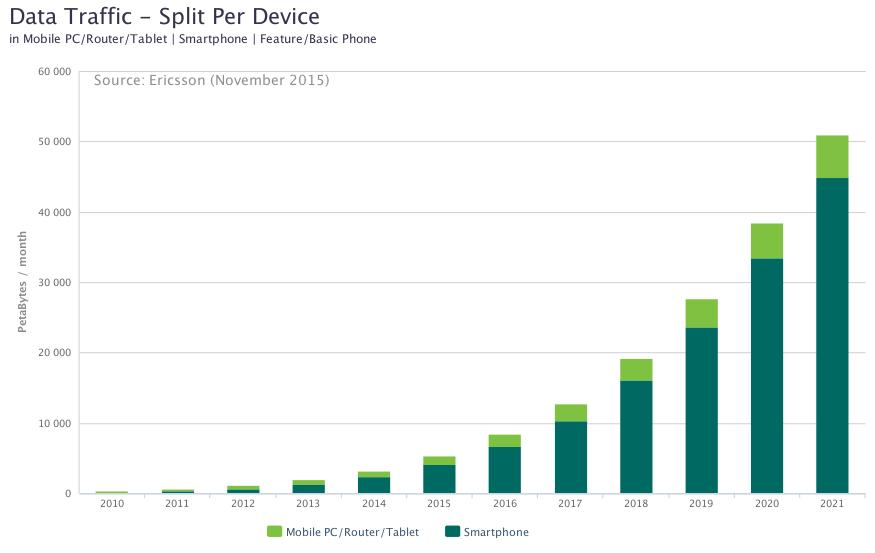
\includegraphics[width=1\textwidth]{1-data-traffic-forecast}
	\caption{Data traffic growth forecast to 2021, as per Ericsson, generated using \cite{ericsson_traffic_exploration}}
	\label{fig:1_data_traffic_forecast}
\end{figure}


\begin{figure}[!tbp]
	\centering
	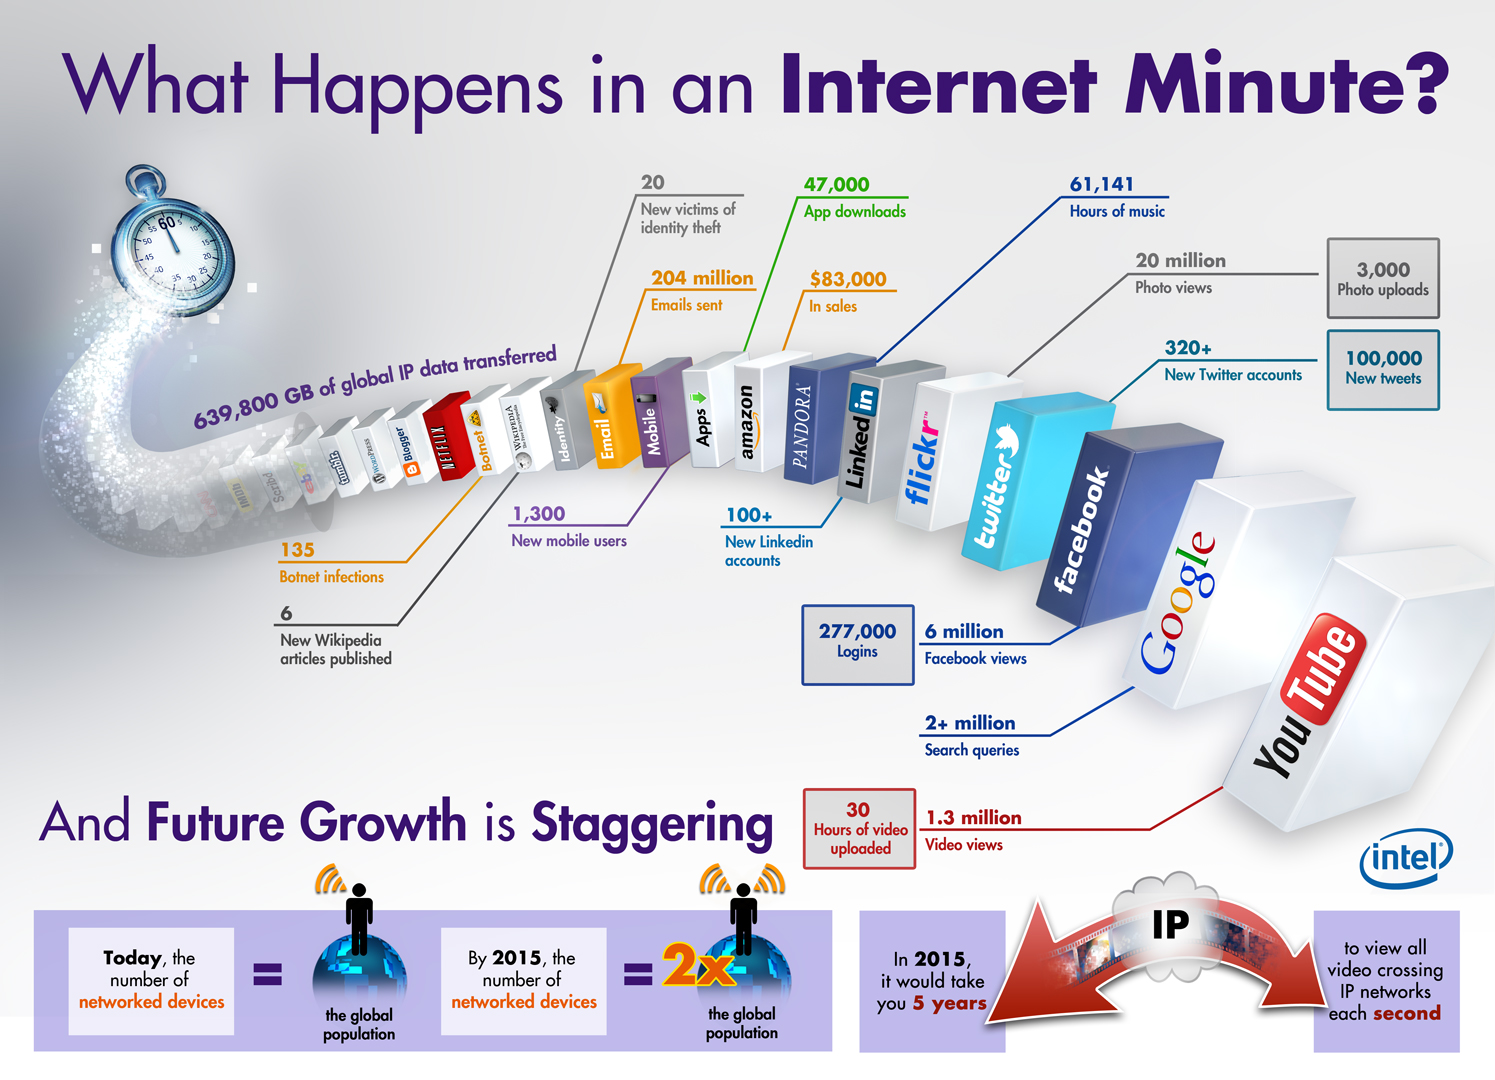
\includegraphics[width=0.80\textwidth]{1-Internet-minute}
	\caption{What happens on internet per minute \cite{internet_minute}}
	\label{fig:1_internet_minute}
\end{figure}
Currently, as illustrated in Fig. \ref{fig:1_internet_minute}, huge data is processed per minute, due to different \gls{ict} services. Eventually, as more and more people use these different \gls{ict} services on different devices, this data growth will be higher than ever. So how is this data traffic managed currently? The answer is the optical fiber based metro and long haul networks, which forms the backbone of the modern communication systems. Optical fiber is chosen over previously used copper cables for the following reasons:
\begin{itemize}
	\item[$\square$] \textbf{Greater bandwidth}: Fiber provides more bandwidth than copper and can transmit up to 100 Gbps and beyond.
	\item[$\square$] \textbf{Reliability and Immunity}: Fiber provides extremely reliable data transmission. It’s completely immune to many environmental factors that affect copper cable such as, electromagnetic and radio-frequency interference, crosstalk and impedance problems.  
	\item[$\square$] \textbf{Security}: Fiber doesn’t radiate signals and is extremely difficult to tap, which provides better security than copper cables.
	\item[$\square$] \textbf{Less attenuation}: Fiber optic transmission results in less attenuation (losses) than copper cables.
	\item[$\square$] \textbf{Lightweight}: Fiber is lightweight, thin, and more durable than copper cable and takes up less space in cable trays.
\end{itemize}

	\section{Silicon photonics}
The performance of optical fiber networks is remarkable and it is this backbone which gives us a great user experience. The current internet architecture has already pushed the optical fiber to the network edges and the trend is to push it as close to the processor as possible. This has already opened up a new trend of “siliconizing photonics” \cite{silicon_photonics}, which arose from the research in microelectronics and photonics industry.\par 
The electronics industry has pushed the boundaries of processing power of \gls{ic} by adding more transistors, according to Moore’s Law. Until recently, the increase in the speed, efficiency, and processing power of conventional electronic devices were achieved largely through clustering and downscaling of components on a chip. However, this trend toward miniaturization has yielded unwanted effects in the form of significant increases in noise, power consumption, signal propagation delay and aggravates already to serious thermal management problems. As a result, traditional microelectronics will soon fall short of meeting market needs, inhibited by the thermal and bandwidth bottlenecks inherent in copper wiring. Comparison in between Intel's processor speed and bus speed shows that although we have achieved good processing speed, the interconnects always find difficulty in catching up with the processing speed \cite{intel_proc_compare}. Annual global data center IP traffic will reach 10.4 zettabytes (863 exabytes per month) by the end of 2019, up from 3.4 zettabytes per year (287 exabytes per month) in 2014 \cite{cisco_forecast_2019}. Think of a server rack in a data center processing an average of this huge data per second, where interconnects between multiple processors in the server rack add up to a significant bottleneck. These bottlenecks can be overcome by substituting copper with optical interconnects, which can also operate at lower power and better efficiency. Additionally, optical interconnects can also improve switching and transmission of electrical signals as well as reduce heat dissipation.\par
Technologies for \gls{oeic} and electronic circuitry can be classified as either hybrid or monolithic. Hybrid integration involves combining optoelectronic devices and \gls{ic} in the same package or substrate. Monolithic integration of GaAs-on-Si is attractive because it would allow one to make use of the wealth of silicon BiCMOS electronics \gls{ic} technology existing today. Unfortunately, III-V epitaxy on silicon (or vice versa) is made difficult by the facts that the lattice constants of GaAs and Si differ by 4\%, and that the thermal expansion coefficients differ by almost 50\%. Although silicon is the material of choice for electronics, only from the late 1980s silicon has been considered a practical option for \gls{oeic} solutions. Silicon has many properties that make it a good material for optics. First of all, the band gap of silicon ($\sim$\SI{1.1}{\electronvolt}) is such that the material is transparent to wavelengths commonly used for optical communication ($\sim$\SI{1.3}{\micro\metre}-\SI{1.6}{\micro\metre}). Moreover, one can use standard \gls{cmos} processing techniques to sculpt optical waveguides onto the silicon surface. Similar to an optical fiber, these waveguides can be used to confine and direct light as it passes through the silicon \cite{reed_silicon_2004} using total internal reflection. Due to the wavelengths typically used for optical transport and silicon’s high index of refraction, the sizes needed for these silicon waveguides are on the order of \SI{0.5}{\micro\metre}-\SI{1}{\micro\metre}. This makes silicon excellent for miniaturization of optical components. The fabrication and lithography requirements needed to process waveguides with these sizes exist today. Finally, it is \gls{cmos}-compatible, making it possible to process monolithic opto-electronic devices, which could bring higher speed, better functionality, power and size reduction, all at a lower cost. Also, recent development in silicon light-emitting diodes \cite{green_efficient_2001} corroborates the usage of silicon for \gls{oeic}. \par

Today, silicon photonics is a new approach to make miniaturized optical devices that use light to move huge amounts of data at very high speeds with extremely low power over a thin optical fiber rather than using electrical signals over a copper wire. Since a large capital investment has already been done on perfecting the current fabrication technology and infrastructure, engineers are working on creating monolithic designs of integrated circuits which will use light instead of electrical signals \cite{optical_linking}. Research institutes and industry, are trying to bridge this gap by creating highly integrated photonic and electronic components that combine the functionality of conventional \gls{cmos} circuits with the significantly enhanced performance of photonic solutions. Various kinds of silicon photonic devices, such as switches \cite{stabile_integrated_2016,wu_mems-enabled_2015,nikolova_scaling_2015,lu_low-power_2014}, modulators \cite{dong_silicon_2015,chen_generation_2013}, photo-detectors \cite{urino_demonstration_2012,chang_high-power_2015}, delay lines \cite{garcia_design_2015,mattarei_variable_2014}, sensors \cite{janz_silicon_2007,lim_laser_2010,ryckeboer_glucose_2014} etc. have been reported to date. This leads to a booming silicon photonics market, which is estimated to grow to 700 million USD by 2024 \cite{jalali_silicon_2006,silicon_photonics_growth_2015} with a \gls{cagr} of 38\%.

	\section{Motivation for MEMS tunable polarization rotator} 
The dynamic control of optical polarization rotation can be utilized to realize a new class of components in integrated photonics including polarization mode modulators, multiplexers, filters, and switches for advanced optical signal processing, coherent communications, and sensing. Advanced sensors can be designed since more spectrometric analysis can be done using tunable modes. Furthermore, the concept can be useful in situations where polarization tuning is necessary under adiabatic conditions; for example in photon entanglement, which promises the development of even smaller micro-electronic devices along with secure communication channels. Moreover, since the power consumption of the \gls{tpr} is very low, this can be used for reconfiguration of network topology at low power. \par

Additionally, to keep up with bandwidth requirements using existing network infrastructure, spatial-division multiplexing techniques \cite{space_richardson_2013} are being contemplated, which uses multi-mode transmission. However, simply connecting the end of such fibers to an \gls{oeic} is far more complicated than standard fibers, because much more mechanical precision is required. Great care has to be taken to make sure light goes in exactly as intended \cite{hecht_is_2016}. Moreover, all photonic devices based on silicon waveguides are sensitive to polarization due to large structural birefringence, which induces substantial \gls{pdl}, \gls{pmd}, and other \gls{pdw}, limiting their usability. Also, in a complex \gls{oeic} system, polarization is a major issue because power can be exchanged between the polarization states in the presence of junctions, tapers, slanted sidewalls, bends, or other discontinuities. Therefore, sometimes, it is necessary to control polarization state, and it may also be necessary to rotate an incoming polarization state. \par

To overcome these challenges, a \gls{pr} is engineered in silicon for \gls{oeic}, and various passive \gls{pr} designs have already been demonstrated \cite{xie_efficient_2015,velasco_ultracompact_2012,leung_numerical_2011,wang_design_2014,dai_novel_2011,wirth_efficient_2012,chen_compact_2011}. However, for dynamic control of optical polarization a \gls{tpr} is required and some designs \cite{sarmiento-merenguel_demonstration_2015, xu_electrically_2014} have also been demonstrated. The tuning is achieved by thermo-optic effect inducing cross-talk problems, which might change phase of the wave in other waveguides in a high density environment, as silicon is highly susceptible to thermal changes \cite{ibrahim_athermal_2012}. Hence, the packing density of these \gls{tpr} using thermo-optic effect is inefficient. Moreover, the \gls{tpr} in \cite{ xu_electrically_2014} uses out-of-plane ring cavity which inherits the narrow band spectral features of ring resonator thus limiting the bandwidth. Hence, the goal of this thesis is to realize an efficient \gls{tpr} with high packing density, using \gls{mems} tuning in C and L bands, at low power, without thermo-optic effect.

	\section{Objectives of the thesis}
\textbf{Main objective}: To design and fabricate a low power \gls{tpr} based on \gls{mems} tuning. \\

\noindent \textbf{Sub objectives}: The areas which will be addressed are:
\begin{itemize}	
	\item[$\square$] Evaluate feasibility of \gls{mems} based \gls{tpr}. 
	\item[$\square$] Design a \gls{mems} \gls{tpr} capable of tuning polarization in between the two fundamental waveguide modes.
	\item[$\square$] Demonstration of the \gls{mems} based \gls{tpr} with an extinction ratio of more than at least \SI{10}{\decibel} for the two fundamental modes, in C and L bands.
\end{itemize}
	
	\section{Outline of this thesis}
The outline of the thesis is as follows: Background, motivation and the research questions being addressed, is discussed in Chapter 1. Background literature of optical waveguide theory is discussed in Chapter 2. In Chapter 3, the current state of art for the available passive and active \gls{pr} solutions are discussed. Here, also the working principle of the current available designs are explained along with the areas which can be improved. Chapter 4 discusses the design of the final system and the simulation results obtained. In Chapter 5, the fabrication details are provided along with the \gls{sem} images of the fabricated product. Experiments and results are discussed in Chapter 6. In Chapter 7, the known limitations of the designed \gls{tpr} are discussed along with future optimizations and work possibilities. Finally, the thesis is concluded with ending remarks in Chapter 8.
	
\end{document}
